%---------------------corebuild------------------------
\chapter{ Corebuild : Construction du système de base}
\label{chap:corebuild}
\minitoc
\clearpage

\section{Introduction}
Les chapitres précédents ont posé les bases théoriques et architecturales de notre distribution. Il est désormais temps de passer à la pratique : ce chapitre marque le début du \textbf{développement concret} de Kraken OS. \\
Son objectif principal réside dans l'intégration sélective des composants critiques indispensables au fonctionnement d'un environnement GNU/Linux autonome.



% -----preparation-----------


\section{Préparation de l’environnement hôte}
\label{subsec:env-hote}

Contrairement au développement d’une application (web, mobile ou logicielle) qui s’appuie sur un IDE, un framework ou des bibliothèques, la construction d’un système d’exploitation requiert un environnement hôte complet. Cet environnement doit fournir shell, compilateur, noyau précompilé,
 utilitaires de base  etc...


Il servira de plateforme temporaire pour assembler notre nouveau système, puis pour y faire un \texttt{chroot} une fois les premières étapes terminées.




\subsection{Configuration logicielle}
on utilise un distribution linux minimale nomme \textbf{archlinux} .
Une vérification préalable des outils de compilation s'impose. Les paquets requis incluent notamment :

\begin{itemize}
    \item \textbf{Outils de base} : Bash, Coreutils, Findutils
    \item \textbf{Chaîne de compilation} : GCC, Binutils, Make
    \item \textbf{Utilitaires système} : Gawk, Grep, Sed
    \item \textbf{Gestion d'archives} : Tar, Xz, Gzip
    \item \textbf{Noyau} : Noyau Linux précompilé. 
\end{itemize}

Une attention particulière est portée aux versions logicielles et aux liens symboliques pour garantir la cohérence des dépendances.


\begin{itemize}  
  \item \textbf{Rôle de ces outils} :  
        Ils seront utilisés pour :  
        \begin{itemize}  
          \item Partitionner le disque destiné au système,  
          \item Créer l’arborescence des systèmes de fichiers,  
          \item Développer le cross-compilateur.  
        \end{itemize}  
  \item \textbf{État final} :  
        À ce stade, nous disposons d’un \textbf{environnement hôte configuré de manière complète}, prêt à construire notre système.  
\end{itemize}  
\textcolor{blue}{Pour plus d’informations sur  la préparation de l’environnement hôte  consultez} \cite{lfs_book} 
 \subsection{Partitionnement du disque}
\label{sssec:partitionnement}

Nous disposons d’un disque temporaire dédié à la construction de la distribution. Il sera monté dans un répertoire spécifique et contiendra notre nouvelle distribution jusqu’à la phase de création de l’image ISO .\\
\textcolor{blue}{Pour en savoir plus sur le partitionnement, les types de disques et les schémas de partitions, reportez‑vous au \cite{archlinux_partition}}.\\



Dans \textsc{Kraken OS}, nous avons choisi ce disque temporaire pour l’ensemble du processus de build. Le schéma de partitionnement adopté respecte les standards UEFI modernes :

\begin{itemize}
  \item \texttt{/dev/sda1} : partition racine (ext4, 150 Go) contenant le système de fichiers ;
  \item \texttt{/dev/sda2} : partition \texttt{/home} (ext4, 100 Go) pour les fichiers et répertoires utilisateurs  ;
  \item \texttt{/dev/sda3} : partition EFI (vfat, 1 Go) ;
  \item \texttt{/dev/sda4} : espace de swap (8 Go).
\end{itemize}
\textbf{Outils utilisés} : \texttt{cfdisk}, \texttt{mkfs.ext4}, \texttt{mkfs.vfat -F 32}, \texttt{mkswap}, \texttt{swapon}, \texttt{mount}, \ldots \texttt{umount}.\\
\noindent\textit{Remarque :} ce disque sera monté en \texttt{/mnt/kraken}.
\begin{itemize}
    
\item \textbf{État final} :  
        À ce stade, le disque dur est :  
        \begin{itemize}  
          \item Correctement configuré (partitionnement, formatage),  
          \item Monté dans notre repertoire cible,  
          \item Prêt à héberger l’arborescence du système.  
        \end{itemize}  
\end{itemize}


\clearpage
\subsection{Hiérarchie du système de fichiers }
\label{sssec:hierarchie-preconfig}

Comme discuté au section \textcolor{blue}{ \ref{sssec:fhs}}, nous restons au plus près du standard FHS (Filesystem Hierarchy Standard).

À ce stade, nous devons créer l’arborescence du système de fichiers \textbf{sur le disque monté}. Cette structure doit correspondre à celle illustrée dans la figure ci-dessous : 

\begin{figure}[H]
  \centering
  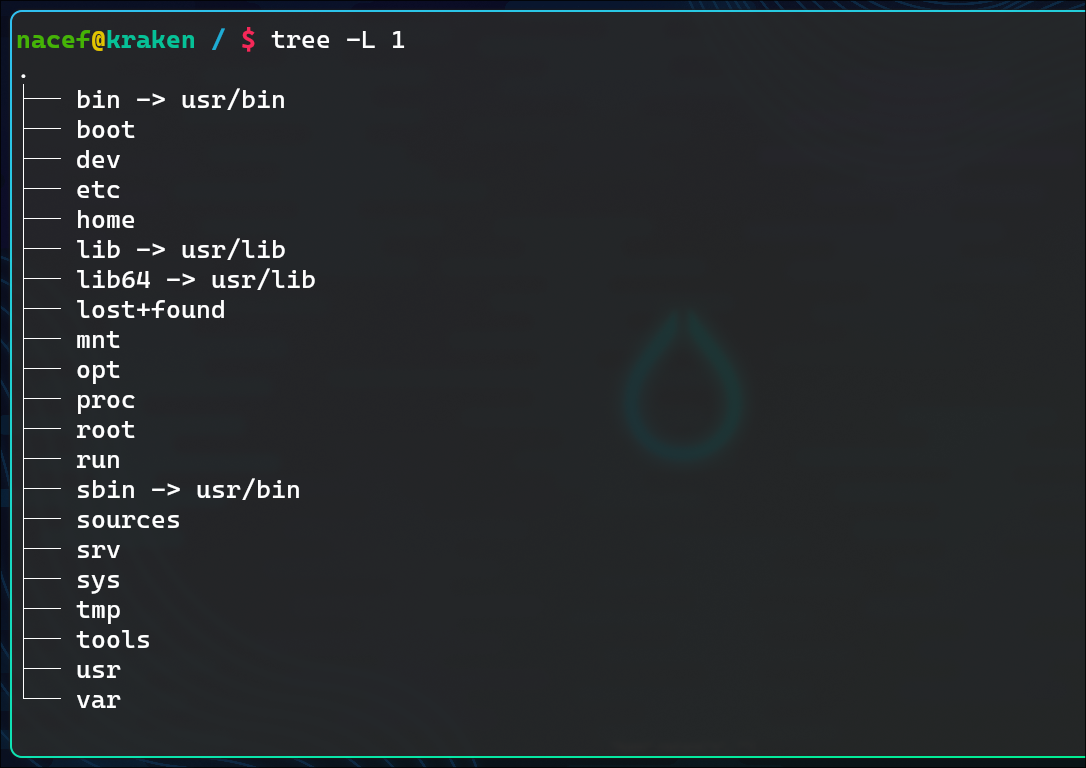
\includegraphics[width=1\textwidth, height=10cm]{images_pfe/minimalfhs.png}
  \caption{Hiérarchie minimale des répertoires conforme au standard FHS}
  \label{fig:minimlfhs}
\end{figure}

\textbf{Remarque :}  
\begin{itemize}
  \item \textbf{Répertoire \texttt{sources}} :  
        Servira à compiler tous les paquets du système.
  \item \textbf{Répertoire \texttt{tools}} :  
        Contiendra le cross-compilateur et sa toolchain.
\end{itemize}

\subsection{Pré-configuration}
Lorsqu’on est connecté en tant que \texttt{root}, une seule erreur peut endommager ou détruire le système. \\Nous devons donc créer un utilisateur dédié et configurer son groupe ainsi que les droits d’accès sur les répertoires et fichiers de l’arborescence. Cet utilisateur sera utilisé pour compiler et configurer les paquets.

\textbf{Outils utilisés}~:  
\texttt{groupadd}, \texttt{useradd}, \texttt{passwd}, \texttt{chown}, \ldots 

Nous devons également ajouter des configurations supplémentaires relatives aux options de compilation et à l’environnement pour préparer le développement de notre compilateur croisé.\\
\clearpage
Exemple de configuration du \texttt{.bashrc} :

\begin{verbatim}
set +h
umask 022
KRAKEN=/mnt/kraken
KRAKEN_TGT=x86-64-kraken-linux-gnu
PATH=$KRAKEN/tools/bin:$PATH

\end{verbatim}

\textbf{Explications~:}

\begin{itemize}
    \item \textbf{set +h:} 
          Désactive l'utilisation de la table de hachage (\emph{hash table}) de Bash. 
          L idee est de \textbf{FORCER} Le shell de rechercherer  les exécutables dans le \texttt{PATH}   plutôt que de mémoriser leurs emplacements.

    \item \textbf{umask 022:} 
          Définit les permissions par défaut pour les nouveaux fichiers/répertoires~: 
         

    \item \textbf{KRAKEN=/mnt/kraken~:} 
          Variable pointant vers le disque monté où notre système sera construit.

    \item \textbf{KRAKEN-TGT=x86-64-kraken-linux-gnu~:} 
          Définit la cible du compilateur croisé. Cette configuration est importante permet de simuler un environnement hôte différent, comme détaillé dans la section suivante.

   

    \item \textbf{/mnt/kraken/tools/bin:PATH~:}
            Permet au shell de détecter immédiatement notre compilateur croisé situé dans \texttt{/tools/bin}.
\end{itemize}

\textcolor{blue}{Pour plus d’informations sur  la préparation de l’environnement hôte  consultez \cite{lfs_book} }









% ----- Compilation croisée -----------
\section{Construction du compilateur croisé et des bibliothèques associées}
\label{subsec:build-cross}
Les etapes principales sont:\\
\begin{enumerate}
  \item Developemnt du compilateur croisé.
  \item Utilisation de ce compilateur pour assembler une chaîne d’outils temporaire.
  \item Emploi de cette chaîne d’outils pour bâtir le système final.
\end{enumerate}

\subsection{Compilateur croisé}
Comme discuté dans le chapitre  \ref{subsec:cross-compiler} sur la compilation, nous devons créer un compilateur croisé «~factice~».  




\subsubsection{Concept clé~: le triplet système}  
Le système de construction basé sur \texttt{autoconf} utilise un format \texttt{cpu-vendor-kernel-os} (appelé «~triplet système~»).

%\textbf{Remarque~:} Si vous vous interrogez sur l’appellation «~triplet~» pour une structure à quatre composants,  voir la section~\hyperref[sec:triplet]{\textcolor{blue}{\ref*{sec:triplet}}} de l'annexe. 

%\subsubsection{Implémentation du compilateur factice}  
Pour simuler le compilateur croisé~:  
\begin{itemize}  
  \item Il faut Modifiez la cible (\texttt{--target}) durant la compilation des paquets~;  
  \item \textbf{Spécifiquement}~: le champ \texttt{vendor}  du triplet système.  
  \begin{itemize}  
    \item Cette approche indique au compilateur d’installer les paquets dans un emplacement différent (\texttt{/mnt/kraken}) plutôt que sur le système hôte.  
  \end{itemize}  
  \item Ajoutez l’option \texttt{--with-sysroot=/mnt/kraken}~:  
  \begin{itemize}  
    \item Force le compilateur à rechercher les bibliothèques \textbf{uniquement} dans notre système (\texttt{/mnt/kraken}),  
    \item Garantit qu’il ne lie \textbf{aucune bibliothèque} du système hôte.  
  \end{itemize}  
\end{itemize}  


Ce compilateur croisé est composé des paquets suivants~:

\begin{table}[H]
    \centering
    \begin{tabular}{|c|p{8cm}|}
        \hline
        \textbf{Paquet}  & \textbf{Fonction principale} \\
        \hline
       GCC                & Compilateur C/C++ (base de la chaîne d’outils) \\
        \hline
        Binutils             & Fournit l’éditeur de liens (\texttt{ld}) et le vérificateur de dépendances (\texttt{ldd}). \\
        \hline
        Linux-API Headers         &   En-têtes du noyau Linux (nécessaires pour la compilation des bibliothèques système). \\
        \hline
        Glibc          & Bibliothèque C GNU (implémente les fonctions de base comme \texttt{printf}, \texttt{malloc}, etc.) etc.) \\
        \hline
        Libstdc++       & Bibliothèque standard C++ (fournit \texttt{std::string}, \texttt{std::vector}, etc.). \\
       
       
        \hline
    \end{tabular}
    \caption{Composants du compilateur croisé}
    \label{tab:crosscompiler}
\end{table}

%\begin{table}[H]
%    \centering
%    \begin{tabular}{|c|c|p{8cm}|}
%        \hline
%        \textbf{Paquet} & \textbf{Version} & \textbf{Fonction principale} \\
%        \hline
%       GCC             & 14.2.0    & Compilateur C/C++ (base de la chaîne d’outils) \\
%        \hline
%        Binutils        & 2.44       & Fournit l’éditeur de liens (\texttt{ld}) et le vérificateur de dépendances (\texttt{ldd}). \\
%        \hline
%        Linux-API Headers         &6.13.4    &   En-têtes du noyau Linux (nécessaires pour la compilation des bibliothèques système). \\
%        \hline
%        Glibc      & 2.41       & Bibliothèque C GNU (implémente les fonctions de base comme \texttt{printf}, \texttt{malloc}, etc.) etc.) \\
 %       \hline
 %       Libstdc++     & 3.10      & Bibliothèque standard C++ (fournit \texttt{std::string}, \texttt{std::vector}, etc.). \\
       
       
 %       \hline
 %   \end{tabular}
 %   \caption{Composants du compilateur croisé}
 %   \label{tab:crosscompiler}
%\end{table}

Ces paquets doivent être configurés avec un préfixe et une cible spécifiques~:
\begin{verbatim}
--prefix=/mnt/kraken/tools
--with-sysroot=/mnt/kraken
--target=x86_64-kraken-linux-gnu
\end{verbatim}

\noindent
Exemple de configuration du paquet \texttt{gcc}~:

\begin{verbatim}
../configure                  \
    --target=$KRAKEN_TGT      \
    --prefix=$KRAKEN/tools    \
    --with-sysroot=$KRAKEN    \     
    --disable-libstdcxx       \
    --enable-languages=c,c++
\end{verbatim}

\textbf{Explications~:}
\begin{itemize}
  \item \textbf{\texttt{--disable/--enable}}~: 
        Active/désactive des fonctionnalités spécifiques durant la compilation.
        
  \item \textbf{\texttt{--target=x86\_64-kraken-linux-gnu} et \texttt{--with-sysroot=/mnt/kraken}}~: 
        Simulent un compilateur croisé en redirigeant :
        \begin{itemize}
          \item La cible vers une architecture personnalisée,
          \item La recherche des bibliothèques vers le système isolé.
        \end{itemize}
        
  \item \textbf{\texttt{--prefix=/mnt/kraken/tools}}~: 
        Définit le répertoire d’installation du compilateur croisé.
\end{itemize}


\subsection{Construction des outils temporaires}
\label{subsec:outils-temp}

Cette section décrit la compilation des utilitaires de base à l’aide de notre nouvelle chaîne d’outils croisée.

Les paquets suivants sont construits en mode cross-compile :
\begin{table}[H]
    \centering
    \begin{tabular}{|c|p{8cm}|}
        \hline
        \textbf{Paquet} & \textbf{Fonction principale} \\
        \hline
        M4               & Traitement des macros dans le code source \\
        \hline
        Ncurses             & Gestion avancée de l’affichage en terminal \\
        \hline
        Bash              & Interpréteur de commandes principal \\
        \hline
        Coreutils             & Commandes système de base (\texttt{ls}, \texttt{cd}, \texttt{mkdir}, etc.) \\
        \hline
        Diffutils            & Comparaison de fichiers et de répertoires \\
        \hline
        File                & Identification du type de fichiers \\
        \hline
        Grep              & Recherche de motifs dans les fichiers \\
        \hline
        Make               & Automatisation des processus de compilation \\
        \hline
        Gettext              & Utilitaires pour l’internationalisation et la localisation \\
        \hline
        Bison              & Générateur d’analyseurs (parser) \\
        \hline
        Perl              & Langage pratique d’extraction et de rapports \\
        \hline
        Python           & Environnement de développement Python \\
        \hline
        Texinfo             & Programmes pour lire, écrire et convertir des pages \texttt{info} \\
        \hline
        Util-linux        & Divers utilitaires système \\
        \hline
    \end{tabular}
    \caption{Chaîne d’outils essentielle}
    \label{tab:toolchain}
\end{table}

%\begin{table}[H]
 %   \centering
 %   \begin{tabular}{|c|c|p{8cm}|}
 %       \hline
 %       \textbf{Paquet} & \textbf{Version} & \textbf{Fonction principale} \\
 %       \hline
 %       M4             & 1.4.19    & Traitement des macros dans le code source \\
 %       \hline
 %       Ncurses        & 6.5       & Gestion avancée de l’affichage en terminal \\
 %       \hline
 %       Bash           & 5.2.32    & Interpréteur de commandes principal \\
 %       \hline
     %   Coreutils      & 9.5       & Commandes système de base (\texttt{ls}, \texttt{cd}, \texttt{mkdir}, etc.) \\
    %    \hline
    %    Diffutils      & 3.10      & Comparaison de fichiers et de répertoires \\
    %    \hline
    %    File           & 5.45      & Identification du type de fichiers \\
    %    \hline
    %    Grep           & 3.11      & Recherche de motifs dans les fichiers \\
    %    \hline
    %    Make           & 4.4.1     & Automatisation des processus de compilation \\
    %    \hline
    %    Gettext        & 0.24      & Utilitaires pour l’internationalisation et la localisation \\
    %    \hline
    %    Bison          & 3.8.2     & Générateur d’analyseurs (parser) \\
    %    \hline
      %  Perl           & 5.40.1    & Langage pratique d’extraction et de rapports \\
      %  \hline
      %  Python         & 3.13.2    & Environnement de développement Python \\
      %  \hline
      %  Texinfo        & 7.2       & Programmes pour lire, écrire et convertir des pages \texttt{info} \\
      %  \hline
      %  Util-linux     & 2.40.4    & Divers utilitaires système \\
      %  \hline
    %\end{tabular}
    %\caption{Chaîne d’outils essentielle}
    %\label{tab:toolchain}
%\end{table}

Exemple dinstallation du paquete M4 :

\begin{verbatim}
    ./configure --prefix=/usr   \
            --host=x86_64-kraken-linux-gnu \
            
        && 
        make
         &&
        make DESTDIR=/mnt/kraken install    
\end{verbatim}


\section{Installation des logiciels système de base}
\label{subsec:install-base}

À ce stade, nous disposons d’une chaîne d’outils complète et pouvons commencer la construction effective de \textsc{Kraken OS}. Les paquets compilés ici sont les versions finales du système. Avant leur installation, il est nécessaire de se placer dans l’environnement chroot correspondant.




\subsection{Chroot vers le nouveau système}
\label{sssec:chroot}

À ce stade, Nous créons un environnement \texttt{chroot} totalement isolé du système hôte (à l’exception du noyau en cours d’exécution). Pour que cet environnement isolé fonctionne correctement, nous devons monter les systèmes de fichiers virtuels du noyau avant d’y entrer.

\paragraph{Préparation des systèmes de fichiers virtuels}
Dans l’arborescence de montage, nous créons les répertoires suivants :
\begin{verbatim}
/dev
/proc
/sys
/run
\end{verbatim}

\textbf{Explications~:}
\begin{itemize}
  \item \texttt{/proc}~: Interface de communication avec le noyau (processus, paramètres système).
  \item \texttt{/dev}~: Points d’accès aux périphériques matériels.
  \item \texttt{/sys}~: Informations sur le matériel et les pilotes en temps réel.
  \item \texttt{/run}~: Données temporaires volatiles .\\
\end{itemize}
Puis nous montons les systèmes de fichiers du noyau hôte :\\

\begin{verbatim}
mount -vt devpts devpts -o gid=5,mode=0620 /mnt/kraken/dev/pts
mount -vt proc   proc   /mnt/kraken/proc
mount -vt sysfs  sysfs  /mnt/kraken/sys
mount -vt tmpfs  tmpfs  /mnt/kraken/run
\end{verbatim}

\textbf{Explications des montages~:}
\begin{itemize}
  \item \texttt{devpts}~: 
        Système de fichiers des pseudo-terminaux esclaves, essentiel pour les commandes nécessitant un terminal (ex: \texttt{sudo}).
        
  \item \texttt{sysfs}~: 
        Expose les informations matérielles et des pilotes à l’espace utilisateur.
        
  \item \texttt{tmpfs}~: 
        Système de fichiers temporaire en RAM pour les données d’exécution volatiles.
        
  \item \texttt{gid=5, mode=0620}~: 
        \begin{itemize}
          \item \texttt{gid=5}~: Associe le groupe \texttt{tty} (id=5) aux pseudo-terminaux,
          \item \texttt{mode=0620}~: Définit les permissions .
        \end{itemize}
\end{itemize}
\noindent
Une fois ces montages effectués, nous pouvons entrer dans le chroot :

\begin{verbatim}
chroot "/mnt/kraken" /usr/bin/env -i \
  HOME=/root                  \
  PATH=/usr/bin:/usr/sbin     \
  MAKEFLAGS="-j6"      \
  /bin/bash --login
\end{verbatim}
\textbf{Explications des configurations importantes :}
\begin{itemize}
  \item \texttt{chroot "/mnt/kraken" /usr/bin/env -i} :  
        Isole l’environnement en réinitialisant les variables système .



  \item \texttt{MAKEFLAGS="-j6"} :  
        Utilise six cœurs du processeur  pour accélérer la compilation.

  \item \texttt{/bin/bash --login} :  
        Force une session de connexion complète au premier accès du \texttt{chroot}.
\end{itemize}

Avant de débuter l’installation, nous modifions plusieurs configurations critiques dans l’environnement chroot :

\begin{itemize}
  \item \textbf{Création des sous‑répertoires critiques}, par exemple :
    \begin{itemize}
      \item \texttt{/lib/firmware}           : stockage des chargeurs d’amorçage  
      \item \texttt{/etc/sysconfig}          : configurations système  
      \item \texttt{/media/floppy, cdrom}    : points de montage pour supports amovibles  
      \item \texttt{/usr/{,local/}share/\{color,dict,doc,info,locale,man\}} : documentation et données partagées  
      \item \texttt{/var/\{cache,local,log,mail,opt,spool\}}             : fichiers variables  
    \end{itemize}

  \item \textbf{Création de liens symboliques essentiels} :
    \begin{itemize}
      \item \texttt{/proc/self/mounts} → \texttt{/etc/mtab}  
      \item \texttt{/var/run}           → \texttt{/run}  
    \end{itemize}
\end{itemize}









\subsection{Compilation et installation des paquets système finaux avec notre chaîne d’outils}
\label{sssec:install-final}

Nous entrons maintenant dans la phase finale de construction, avec l’installation des 80 paquets fondamentaux :
\begin{table}[H]
\centering
\begin{tabular}{|l|l|}
\hline
\textbf{Catégorie} & \textbf{Exemples de paquets} \\
\hline
Noyau et bas niveau & Glibc, Binutils, GCC \\
\hline
Compression et archivage & Zlib, Xz \\
\hline
Outils de compilation & Make, Autoconf, Meson, Flex \\
\hline
Langages et développement & Python, Perl \\
\hline
Shell et interface utilisateur & Bash, Ncurses, Readline \\
\hline
Utilitaires Unix essentiels & Coreutils, Gawk, Grep \\
\hline
Réseau & IPRoute2, Inetutils \\
\hline
Système de fichiers & Util-linux, Udev \\
\hline
Gestion du système & SysVinit \\
\hline
Documentation & Man-pages, Texinfo \\
\hline
Gestion de paquets & Pkgconf \\
\hline
Chargeur de démarrage & GRUB \\
\hline
\end{tabular}
\caption{Catégories des paquets système finaux}
\label{tab:categories-paquets}
\end{table}



%\begin{itemize}
%    \item \textbf{Noyau et bas niveau} : Glibc-2.40, Binutils-2.43.1, GCC-14.2.0  
%    \item \textbf{Gestion de paquets} : Pkgconf-2.3.0, Dpkg-1.22.6  
%    \item \textbf{Sécurité} : Libcap-2.70, Shadow-4.16.0  
%    \item \textbf{Réseau} : IPRoute2-6.10.0, OpenSSL-3.3.1  
%    \item \textbf{Interface utilisateur} : Ncurses-6.5, Bash-5.2.32  
%\end{itemize}

%Liste complète des paquets critiques :

%\begin{verbatim}
%Man-pages-6.9.1        Iana-Etc-20240806     Glibc-2.40
%Zlib-1.3.1             Bzip2-1.0.8           Xz-5.6.2
%Lz4-1.10.0             Zstd-1.5.6            File-5.45
%Readline-8.2.13        M4-1.4.19             Bc-6.7.6
%Flex-2.6.4             Tcl-8.6.14            Expect-5.45.4
%DejaGNU-1.6.3          Pkgconf-2.3.0         Binutils-2.43.1
%GMP-6.3.0              MPFR-4.2.1            MPC-1.3.1
%Attr-2.5.2             Acl-2.3.2             Libcap-2.70
%Libxcrypt-4.4.36       Shadow-4.16.0         GCC-14.2.0
%Ncurses-6.5            Sed-4.9               Psmisc-23.7
%Gettext-0.22.5         Bison-3.8.2           Grep-3.11
%Bash-5.2.32            Libtool-2.4.7         GDBM-1.24
%Gperf-3.1              Expat-2.6.2           Inetutils-2.5
%Less-661               Perl-5.40.0           XML::Parser-2.47
%Intltool-0.51.0        Autoconf-2.72         Automake-1.17
%OpenSSL-3.3.1          Kmod-33               Libelf (Elfutils-0.191)
%Libffi-3.4.6           Python-3.12.5         Flit-Core-3.9.0
%Wheel-0.44.0           Setuptools-72.2.0     Ninja-1.12.1
%Meson-1.5.1            Coreutils-9.5         Check-0.15.2
%Diffutils-3.10         Gawk-5.3.0            Findutils-4.10.0
%Groff-1.23.0           GRUB-2.12             Gzip-1.13
%IPRoute2-6.10.0        Kbd-2.6.4             Libpipeline-1.5.7
%Make-4.4.1             Patch-2.7.6           Tar-1.35
%Texinfo-7.1            Vim-9.1.0660          MarkupSafe-2.1.5
%Jinja2-3.1.4           Udev                  Man-DB-2.12.1
%Procps-ng-4.0.4        Util-linux-2.40.2     E2fsprogs-1.47.1
%Sysklogd-2.6.1         SysVinit-3.10
%\end{verbatim}


Exemple dinstallation du paquete Flex :

\begin{verbatim}
    ./configure --prefix=/usr \                #Configuration 
            --docdir=/usr/share/doc/flex-2.6.4 \
            
     && 
        make  #Compilation
     &&
        make check   #Test
     &&
         make install  #Installation
     &&
         ln -sv flex   /usr/bin/lex   #Liens symboliques
     &&
         ln -sv flex.1 /usr/share/man/man1/lex.1  #Documentation
\end{verbatim}

\textbf{Remarque :} Ce chapitre est principalement inspiré du livre LFS, que ce soit pour le compilateur croisé, le choix des paquets, leurs versions ou certaines configurations.

\textcolor{blue}{Pour plus d’informations, voir~: \cite{lfs_book}}
 
\section{Conclusion}
À ce stade, nous disposons d’un système minimal fonctionnel. Dans la section suivante, nous verrons la configuration du chargeur d’amorçage, la rédaction des scripts de démarrage et l’intégration du noyau pour rendre le système amorçable.```
\clearpage